%%%%%%%%%%%%%%%%%%%%%%%%%%%%%%%%%%%%%%%
% Header                              %
%%%%%%%%%%%%%%%%%%%%%%%%%%%%%%%%%%%%%%%
% 
% Revisions: 2017-12-12 Martin Raedel <martin.raedel@dlr.de>
%                       Initial draft
%               
% Contact:   Martin Raedel,  martin.raedel@dlr.de
%            DLR Composite Structures and Adaptive Systems
%          
%                                 __/|__
%                                /_/_/_/  
%            www.dlr.de/fa/en      |/ DLR
% 
%%%%%%%%%%%%%%%%%%%%%%%%%%%%%%%%%%%%%%%
% Content                             %
%%%%%%%%%%%%%%%%%%%%%%%%%%%%%%%%%%%%%%%

% \begin{parbox}
\begin{tikzpicture}[
  every node/.style={
    font=\figurefontsize,
  }
]
  % External figure
  \node[anchor=south west,inner sep=0] (image) at (0,0) {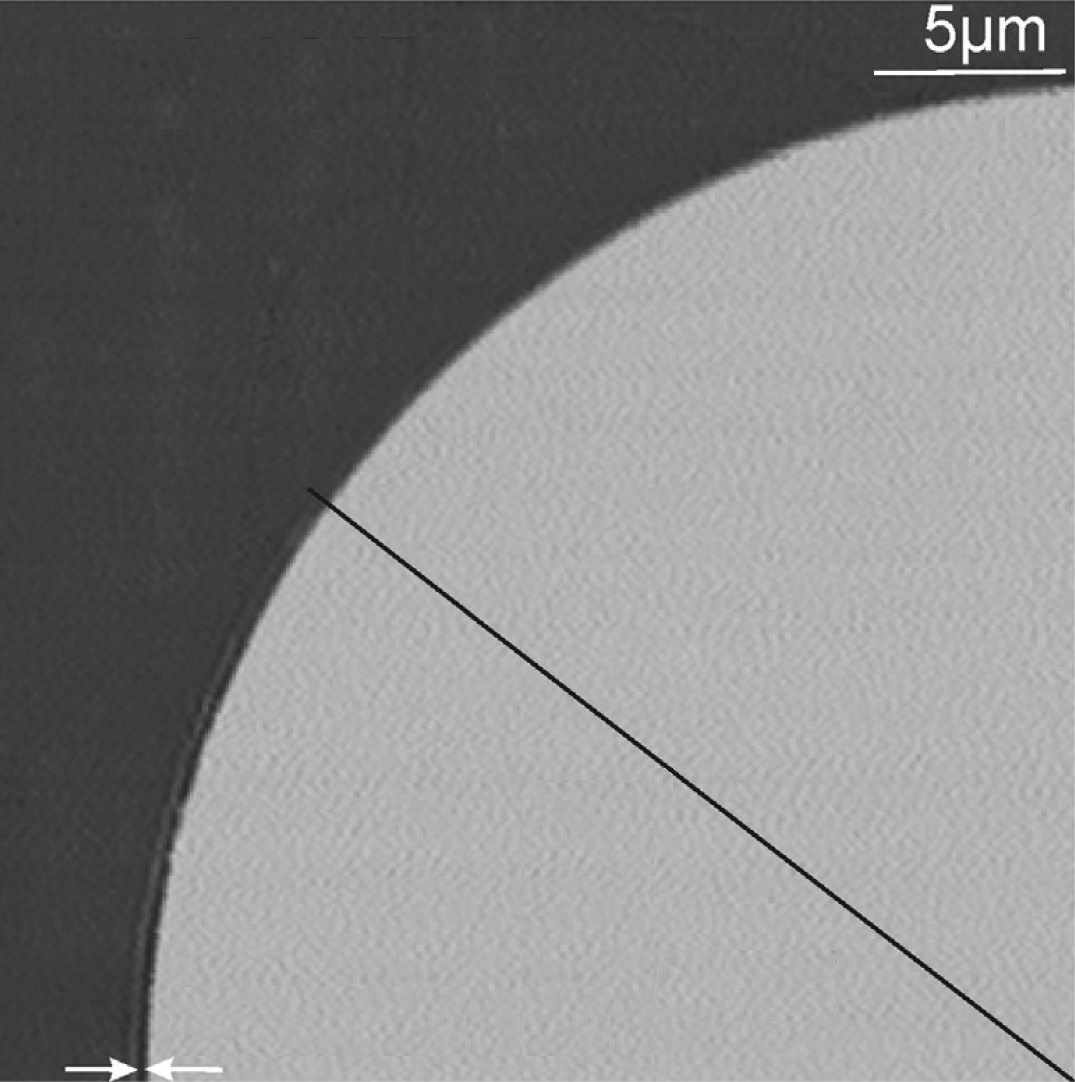
\includegraphics[width=\figwidth,height=\figheight,keepaspectratio]{Exp_Fibre_MartyniukK2013_woLabels2}};
  % Figure scope
  \begin{scope}[
    x={(image.south east)},
    y={(image.north west)},
  ]
    
    \node[anchor=north west,white,inner sep=0pt] (sigmalabel) at (0.025,0.975) {$\glssymbol{symb:scalar:mech:stress:normal:engineering}=\SI{6.2}{\mega\pascal}$};
    
    \node[anchor=south west,black,inner sep=0pt] (deltalabel) at (0.145,0.02) {$\glssymbol{symb:scalar:geo:separation}{=}\SI{0.26}{\micro\meter}$};
    
    %\node[anchor=south east,black,inner sep=0pt] (deltalabel) at (0.85,0.02) {$\glssymbol{symb:scalar:geo:angle:debonding}=\SI{35}{\degree}$};
    
    % This is influenced by the aspect ratio, but since the included graphics is almost square -> hae
    \draw[thin, latex-latex] (1,0) ++(180:0.4) arc (180:142:0.4) node[pos=0.25,right,inner sep=1pt]{$\glssymbol{symb:scalar:geo:angle:debonding}{=}\SI{35}{\degree}$};
    
    % Help grid and labels
    %\pic{myimagegrid};
  \end{scope}
\end{tikzpicture}